\chapter{Design and Implementation}
\label{sec:designandimplementation} 

This chapter presents the design and implementation of StoryBook. It first discusses the authors' journey in dealing with the data in Facebook and the issues inherent in its characteristics. This is followed by the discussion on the event classification algorithm of the system, its issues, initial shortcomings, and improvements. It ends with a discussion of the natural language generation module, which has three submodules: the GenIntro, GenBody, and GenConclusion. The issues encountered during implementation and the solutions applied to address each issue are presented.

%section~~~~~~~~~~~~~~~~~~~~~~~~~~~~~~~~~~~~~~~~~~~~~~~~~~~~~~~~~~~~~~
\section{System Design}
\figref{fig:IAD} shows the system architecture of \systemname.

\begin{figure}[!htb]                %-- use [t] to place figure at top, [b] to place at the bottom, [h] for here
	\centering                    %-- use this to center the figure
	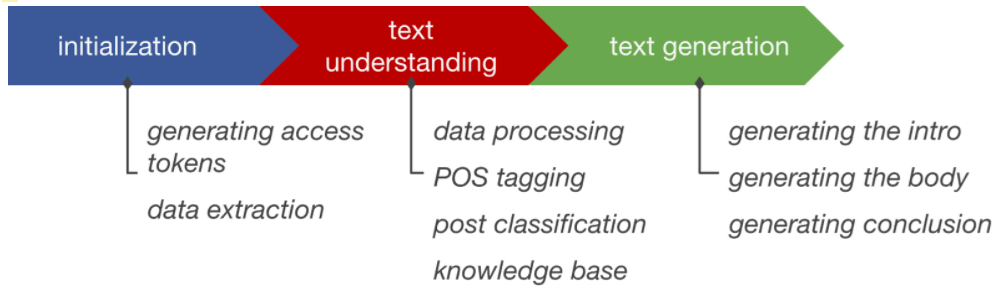
\includegraphics [width=\textwidth] {IAD.png}      %-- include image file named as "disneychart.png" 
	\caption{System Architecture of \systemname}
	\label{fig:IAD}
\end{figure}

\subsection{Initialization}
\textit{Part of: Startup} \newline \newline
The user, via the use of the Facebook Login API \cite{FacebookLogin}, must give his/her login credentials to allow their Facebook data to be extracted for use. After the user goes through each of the permissions and allows them, Facebook generates an access token, which is then used by Graph API to determine which data can be extracted from the Facebook account of the user.

\subsection{Data Extraction}
\textit{Part of: Text Understanding} \newline \newline
This uses Graph API. Three types of data need to be extracted and partitioned into: [1] personal info that can be used as is, such as the user's birthday and list of family members; [2] data which have to be processed such as posts; and [3] the user's list of preferences and events attended. 

The partitioned data will be stored in seven separate tables: direct\_knowledge, educational\_bg, work, family, to\_be\_processed, likes and events, as shown in \figref{fig:ExtractedDataDB}. 

\begin{figure}[!htb]                %-- use [t] to place figure at top, [b] to place at the bottom, [h] for here
	\centering                    %-- use this to center the figure
	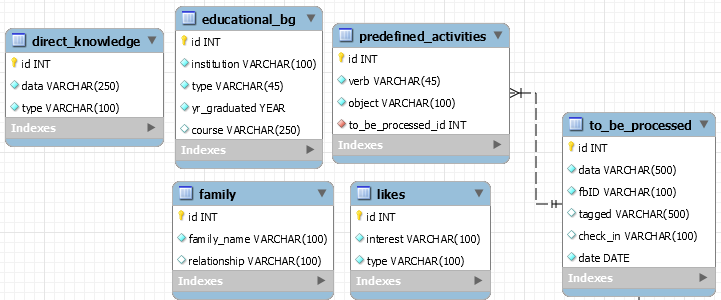
\includegraphics [width=\textwidth] {ExtractedDataDB2.png}      %-- include image file named as "disneychart.png" 
	\caption{Database Design for Storing Extracted Data.}
	\label{fig:ExtractedDataDB}
\end{figure}

Direct knowledge can be extracted from Facebook's About Me section, which contains the personal information of the user. The extracted data also known as the direct knowledge or facts about the user are stored in the \textit{Direct Knowledge Table} (Table \ref{tab:DirectKnowledge}), which contains the following fields:
\begin{itemize}
	\item id - unique value that identifies each fact
	\item data - the direct knowledge data extracted from his/her Facebook account
	\item type - the type of knowledge that describes the data
\end{itemize}
See Appendix \ref{sec:appendixi} for the complete list of types available and a description of each.

Given the sample \textit{About Me} section of a user in Facebook (\figref{fig:AboutMe}), some of the data are shown in Table \ref{tab:DirectKnowledge}:

\clearpage
\begin{figure}[!htb]                %-- use [t] to place figure at top, [b] to place at the bottom, [h] for here
	\centering                    %-- use this to center the figure
	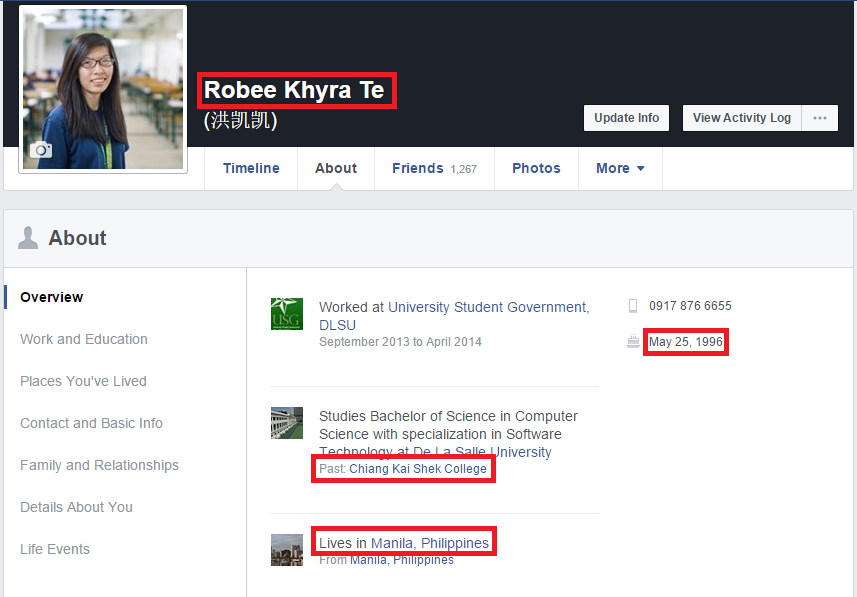
\includegraphics [width=6in,height=4in,keepaspectratio] {AboutMe.png}      %-- include image file named as "disneychart.png" 
	\caption{Sample About Me Section in Facebook}
	\label{fig:AboutMe}
\end{figure}

\begin{table}[ph!]   %t means place on top, replace with b if you want to place at the bottom
	\centering
	\caption{Sample data in the direct\_knowledge table.} \vspace{0.25em}
	\begin{tabular}{|p{1.5cm}|p{2in}|p{1.5in}|} \hline
		\textbf{id} & \textbf{data} & \textbf{type} \\ \hline
		1 & Robee Khyra Te & name \\ \hline
		2 & NULL & middle\_name \\ \hline
		3 & Te & last\_name \\ \hline
		4 & 1996-05-25 & birth\_date \\ \hline
		5 & Manila, Philippines & location \\ \hline
	\end{tabular}
	\label{tab:DirectKnowledge}
\end{table}

The educational background of the user can also be extracted from Facebook's \textit{About Me} section. These are then stored in the \textit{Educational Background Table} (Table \ref{tab:EducationalBG}), which contains the following fields:
\begin{itemize}
	\item id - unique value that identifies each educational level
	\item institution - the name of the institution
	\item type - the type of educational level
	\item year\_graduated - year graduated or ended in the institution
	\item course - course taken in the said institution
	\item fbID - unique id generated by Facebook for each institution
\end{itemize}
See Appendix \ref{sec:appendixi} for the complete list of types available and description of each.

\begin{table}[ph!]   %t means place on top, replace with b if you want to place at the bottom
	\centering
	\caption{Sample data in the educational_bg table.} \vspace{0.25em}
	\begin{tabular}{|p{.5cm}|p{1in}|p{1.5cm}|p{2cm}|p{2.5cm}|p{2cm}|} \hline
		\textbf{id} & \textbf{institution} & \textbf{type} & \textbf{year\_ \newline graduated} & \textbf{course} & \textbf{fbID} \\ \hline
		1 & De La Salle University & College & null & Bachelor of Science in Computer Science with specialization in Software Technology &  \\ \hline
		2 & Chiang Kai Shek College & High School & 2013 & null & \\ \hline
	\end{tabular}
	\label{tab:EducationalBG}
\end{table}

Current or previous work of the user can also be extracted from Facebook's About Me section. These are then stored in the \textit{Work Table} (Table \ref{tab:work}), which contains the following fields:
\begin{itemize}
	\item id - unique value that identifies each work
	\item institution - the name of the institution
	\item date\_started - year started working in the institution
	\item date\_ended - year ended working in the institution
	\item location - location of the said institution
	\item fbID - unique id generated by Facebook for each work institution
\end{itemize}

\begin{table}[ph!]  
	\centering
	\caption{Sample data in the work table.} \vspace{0.25em}
	\begin{tabular}{|p{.5cm}|p{1.5in}|p{2cm}|p{2cm}|p{2cm}|p{2.5cm}|} \hline
		\textbf{id} & \textbf{institution} & \textbf{date\_ \newline started} & \textbf{date\_\newline ended} & \textbf{location} & \textbf{fbID} \\ \hline
		1 & University Student Government, DLSU & 2013-09-01 & 2014-04-30 & Manila, Philippines &  
		3459628907221
		\\ \hline
	\end{tabular}
	\label{tab:work}
\end{table}

Family members of the user can also be extracted from Facebook's \textit{About Me} section. These are then stored in the \textit{Family Table} (Table \ref{tab:Family}), which contains the following fields:
\begin{itemize}
	\item id - unique value that identifies each family member
	\item family\_name - name of the family member
	\item relationship - relationship with the user
	\item fbID - unique id generated by Facebook for each family member
\end{itemize}
See Appendix \ref{sec:appendixi} for the complete list of available relationships.

\begin{table}[ph!]   %t means place on top, replace with b if you want to place at the bottom
	\centering
	\caption{Sample data in the family table.} \vspace{0.25em}
	\begin{tabular}{|p{1.5cm}|p{2in}|p{1.5in}|} \hline
		\textbf{id} & \textbf{family\_name} & \textbf{relationship} & \textbf{fbID} \\ \hline
		1 & Jennilyn Wang & sister & \\ \hline
		2 & Renee Te & sister & \\ \hline
	\end{tabular}
	\label{tab:Family}
\end{table}

Data taken from the user's posts, on the other hand, requires further processing.

The assumptions for these posts are:
\begin{enumerate} [label=\alph*.]
	\item They all contain a text portion;
	\item The created time of the original post (in case there were no edits made) is assumed to be the time the event happened;
	\item If there were edits made, the edited time would be used and considered to determine the time sequence of the posts;
	\item The people tagged are used to know that those people are with the user at the time of the event; and
	\item All content provided are correct.
\end{enumerate}

\clearpage
\begin{figure}[!htb]                %-- use [t] to place figure at top, [b] to place at the bottom, [h] for here
	\centering                    %-- use this to center the figure
	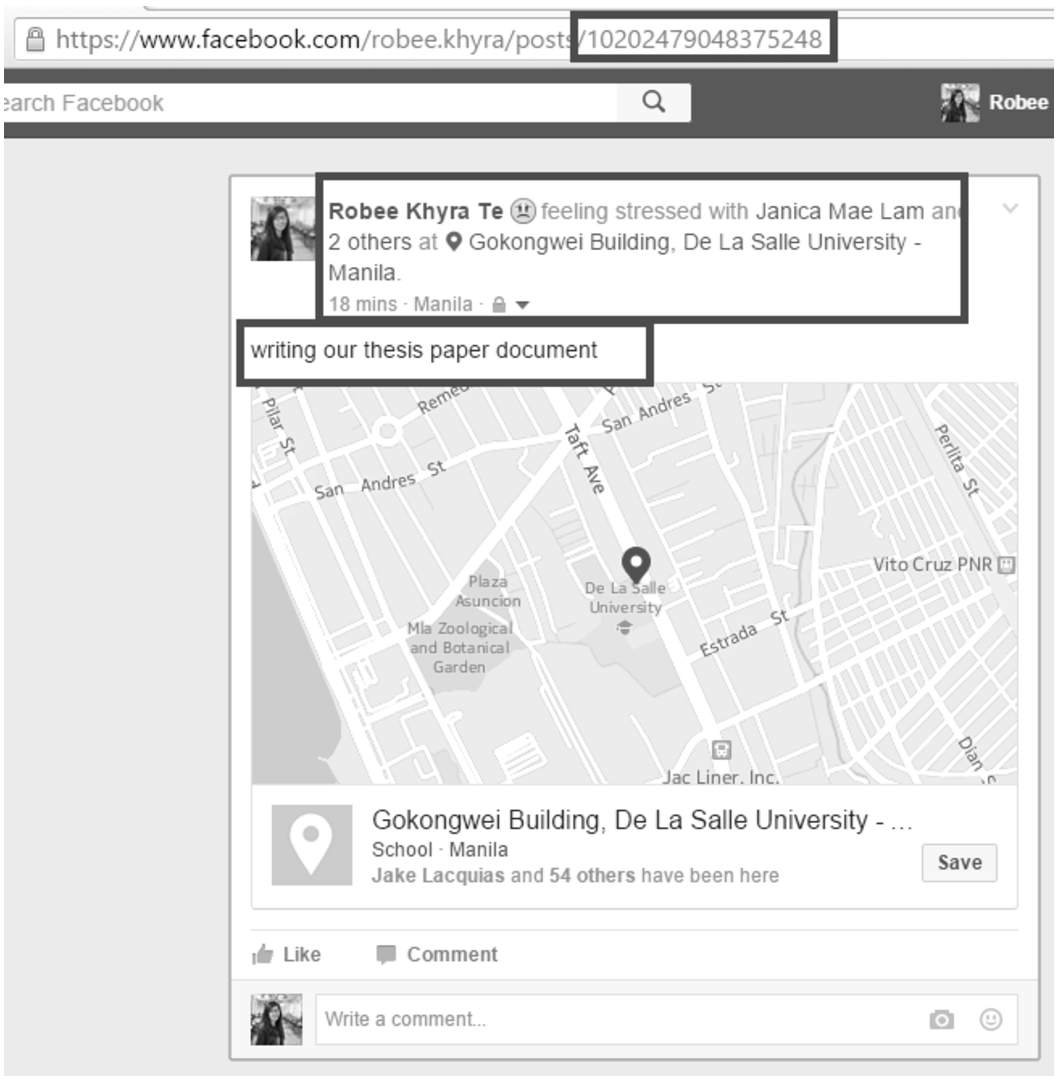
\includegraphics [width=5in,height=4in,keepaspectratio] {SamplePost.png}      %-- include image file named as "disneychart.png" 
	\caption{Sample Post in Facebook}
	\label{fig:SamplePost}
\end{figure}

The \textit{To Be Processed Table} (Table \ref{tab:ToBeProcessed}) is used to store the description or caption in the user's status and posts, including other relevant information regarding the posts. The following are the attributes of the \textit{To Be Processed} table:
\begin{itemize}
	\item id - unique value that identifies each post
	\item data - the description/caption extracted from his/her Facebook account
	\item fbID - unique id generated by Facebook for each post
	\item tagged - comma-separated values representing the friends the user is with for each post
	\item place - the place where the event happened
	\item city - the city where the event happened
	\item country - the country where the event happened
	\item year - the year when the post was created
	\item month - the month when the post was created
	\item day - the day when the post was created
\end{itemize}

\begin{table}[ph!]   %t means place on top, replace with b if you want to place at the bottom
	\centering
	\caption{Sample data in the to\_be\_processed table.} \vspace{0.25em}
	\begin{tabular}{|p{1cm}|p{1in}|p{1in}|p{1in}|p{2cm}|p{1.5cm}|} \hline
		\textbf{id} & \textbf{data} & \textbf{fbID} & \textbf{tagged} & \textbf{check\_in} & \textbf{date} \\ \hline
		1 & writing our thesis paper document & 102024790 \newline 48375248 & Janica Mae Lam, Camille Saavedra, Alds Hade & Gokongwei Building, De La Salle University - Manila & 2016-11-22 \\ \hline
	\end{tabular}
	\label{tab:ToBeProcessed}
\end{table}

Given the sample list of user's liked pages section in Facebook (\figref{fig:LikedPage}), the liked data that are stored in the database is shown in Table \ref{tab:Likes}.

\begin{figure}[!htb]                %-- use [t] to place figure at top, [b] to place at the bottom, [h] for here
	\centering                    %-- use this to center the figure
	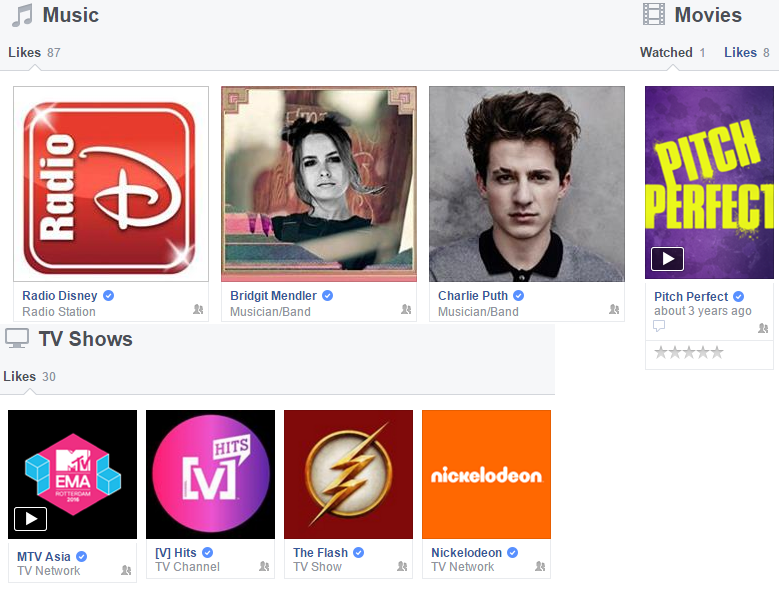
\includegraphics [width=5in,height=4in,keepaspectratio] {LikedPage.png}      %-- include image file named as "disneychart.png" 
	\caption{Sample Interest Preference in Facebook}
	\label{fig:LikedPage}
\end{figure}

The \textit{Likes Table} (Table \ref{tab:Likes}) contains the interest preferences of a particular user in Facebook. This also specifies what time of interest it is.
\begin{itemize}
	\item id - unique value that identifies each interest
	\item interest - the specific interest liked by the user in his/her Facebook account
	\item type - the type of interest that describes the interest
	\item fbID - unique id generated by Facebook for ech page
\end{itemize}
See Appendix \ref{sec:appendixi} for the complete list of available types.

\begin{table}[ph!]   %t means place on top, replace with b if you want to place at the bottom
	\centering
	\caption{Sample data in the likes table.} \vspace{0.25em}
	\begin{tabular}{|p{1.5cm}|p{2in}|p{1.5in}|} \hline
		\textbf{id} & \textbf{data} & \textbf{type} \\ \hline
		1 & Radio Disney & 121 (Radio Station) \\ \hline
		2 & Bridgit Mendler & 93 (Musician/Band) \\ \hline
		3 & Charlie Puth & 93 (Musician/Band) \\ \hline
		4 & Pitch Perfect & 91 (Movie) \\ \hline
		5 & MTV Asia & 147 (TV Network) \\ \hline
		6 & [V] Hits & 146 (TV Channel) \\ \hline
		7 & The Flash & 149 (TV Show) \\ \hline
		8 & Nickelodeon & 147 (TV Network) \\ \hline
	\end{tabular}
	\label{tab:Likes}
\end{table}

Given the sample list of user's going and interested events in Facebook \figref{fig:events}, the events data that are stored in the database is shown in Table \ref{tab:events1}.

The \textit{Events} table (Table \ref{tab:events1}) contains all the going and interested events of a particular user in Facebook. It contains the following fields:
\begin{itemize}
	\item id - unique value that identifies each interest
	\item name - the specific interest liked by the user in his/her Facebook account
	\item rsvp\_status - the type of interest that describes the interest 
	\item place - the place where the event took place
	\item city- the city where the event took place
	\item country - the country where the event took place
	\item fbID - unique id generated by Facebook for each event
\end{itemize}
See Appendix I for the complete list of types available.
\clearpage

\subsection{Inferencing}
\textit{Part of: Text Understanding} \newline \newline
Some user interests have to be inferred, to answer questions such as, ``how does one determine if one likes music?” This particular question can be answered by looking at the list of a person's liked pages.

Facebook has six (6) general categories for Pages, and around 100 specific categories. For this study, the top five categories with the most liked pages by the user are written down in the story. Narrowing down the categories to the top five allows the life story to focus on the things that the user likes the most.

For instance, if the user likes 87 pages of the category ``Musician/Band” and it falls under the top five categories of pages she has liked, it can be inferred that she likes music. The top five categories are later used in the conclusion. 2-3 sample pages under each category are used in the to provide support.

\subsection{Data Processing}
\textit{Part of: Text Understanding} \newline \newline
This process utilizes Stanford CoreNLP. For those data from which knowledge cannot be easily inferred, a more specific procedure of text understanding algorithms is applied. Data preprocessing processes the input and stores them in an abstract representation for use by other modules of \systemname. Hashtags, hyperlinks, emoticons, laughter, and foreign characters are removed from posts before undergoing text understanding, in order to lessen misclassifications.

After the text has been preprocessed accordingly, different event details such as the noun phrase and verb phrase can now be identified. Stanford CoreNLP splits a post into sentences, and for each sentence, syntax analysis is performed.

The direct objects, the lemmatized verb, as well as other information that were extracted directly from Facebook earlier such as the date of the post, location of the event, and people whom the user is with at the time of the post are then stored in the \textit{Verb Object Table} (shown in Table \ref{tab:sampleVO}) to be used later for the generation of body.

The \textit{Verb Object} table (Table \ref{tab:sampleVO}) contains all the event details in a particular post. It contains the following fields:
\begin{itemize}
	\item id - unique value that identifies each interest
	\item post\_id - value (corresponding to the id from the to\_be\_processed table) representing the post where the sentence is taken from 
	\item verb - the identified verb of the post
	\item noun - the identified object of the post
	\item sentence - an individual sentence from the original post
	\item post\_type - value (corresponding to the id from the post\_type table) representing the post type of the sentence
	\item tagged - the people tagged in the post acquired from the to\_be\_processed table
	\item location - the location where the event took place acquired from the to\_be\_processed table
	\item date - the date when the event happened acquired from the to\_be\_processed table
\end{itemize}
\clearpage
\begin{table}[ph!]   
	\centering
	\caption{Sample data in the verb object table.} \vspace{0.25em}
	\begin{tabular}{|p{1cm}|p{1in}|p{1.5cm}|p{1in}|p{1in}|} \hline
		\textbf{id} & \textbf{post\_id} & \textbf{verb} & \textbf{noun} & \textbf{sentence}\\ \hline
		1&1&write&thesis paper document&writing our thesis paper document \\ \hline
	\end{tabular}
	\label{tab:sampleVO}
\end{table}

\begin{table}[ph!]   
	\centering
	\begin{tabular}{|p{1in}|p{1in}|p{1in}|p{1in}|} \hline
		\textbf{post\_type} & \textbf{tagged}& \textbf{location} & \textbf{date}\\ \hline
		&Janica Mae Lam, Camille Saavedra, Alds Hade&Gokongwei Building, De La Salle University& 11/22/2016 \\ \hline
	\end{tabular}
\end{table}

Notice that the post\_type is currently empty because the post still needs to undergo the post classification module. In cases that the Stanford CoreNLP cannot determine a verb or a noun from the given post, the column verb or noun will also be empty. Also, the columns tagged and location can also be empty, if there are no data supplied by the user.

\begin{figure}[!htb]                %-- use [t] to place figure at top, [b] to place at the bottom, [h] for here
	\centering                    %-- use this to center the figure
	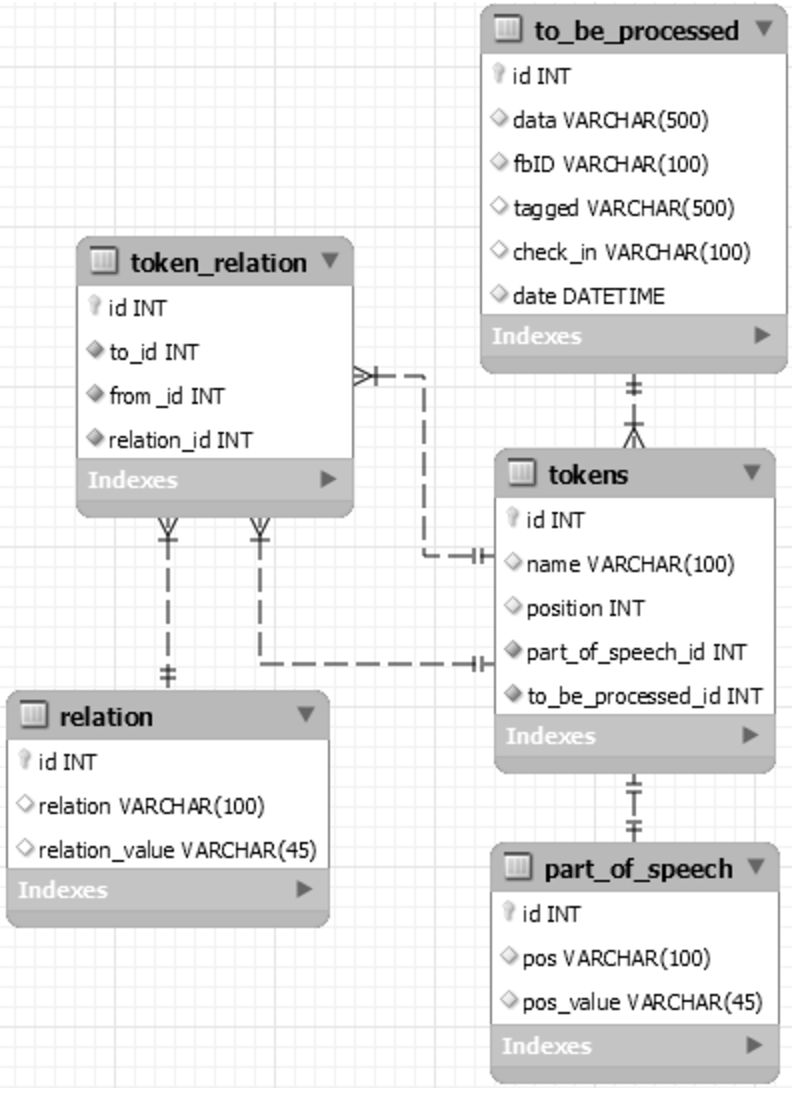
\includegraphics [width=3in,height=3in,keepaspectratio] {dbdesign.png}      %-- include image file named as "disneychart.png" 
	\caption{Database design for storing the processed data.}
	\label{fig:dbdesign}
\end{figure}

\subsection{Knowledge Base}
\textit{GenIntro}, \textit{GenBody}, and \textit{GenConclusion}, which will be discussed in 5.1.6, uses grammar rules and assertions in order to generate the story. These are stored in the database. 

\subsection{Text Generation}
The text generation module is responsible for generating the appropriate story segments that make up the entire life story generated by \systemname. The tool, SimpleNLG, is used for text generation.

There are three components of the text generation modules, namely the GenIntro, GenBody, and GenConclusion. GenIntro is applied to the data determined to be ``facts'' or direct knowledge. The generated text will become the introductory paragraph of the life story.

GenBody is applied to generate the body of the life story from the data processed in the Data Processing module. The body paragraph(s) will be narrating one or more events about a person's life. These events will be taken from data that users have written and posted on their own Timeline. For these data, text generation is more complex. It will undergo three sub-modules, which are all detailed in Section 3.5.1, Text Generation. Each activity in each sub-module is discussed below.

From the data forwarded by the Pre-Processing module, content determination will now classify all the verbs stored in the \textit{Verb Object} table according to type (e.g. all ``eating” together, then all ``travelling to”, then all ``celebrating”). Because a single post can contain multiple verbs or words signifying events, it can be classified into multiple categories. For example, the post, ``\textit{walking around the streets of Rome while eating delicious gelato.}” is classified as eating and travelling.

From the given sample post above, the verb is identified to be ``write”. To be able to determine the post type, it will check the \textit{Post Type} table for the corresponding id of the verb and update the post\_type column in the \textit{Verb Object} table. After the post classification module, the \textit{Verb Object} table (shown in Table  \ref{tab:sampleUpVO}) now contains the updates data.

However, in case of there is no verb present in the post, a reference table (shown in Appendix \ref{sec:appendixl}) containing predefined keywords commonly associated with each event category that was derived through manual inspection of the dataset will be used to classify the post type. For \textit{celebrating} events, words which usually indicate special events such as birthdays and Christmas are used. For posts on \textit{travelling}, synonyms as well as methods of traveling are used. For \textit{eating}, aside from synonyms, the meals of the day are also used as indicators.

All post types stored in the \textit{Verb Object} table are first sequenced according to date. For every classified post in the Verb Object table (Table \ref{tab:sampleVO}), content determination constructs a message for each of it. Each constructed message consists of the object from the Verb Object table pertaining to the said verb together with whom, when and where the event has happened.

With the sample event in \textit{Verb Object} table (Table \ref{tab:sampleUpVO}), content determination can generate the message \textit{write(Robee Khyra Te, thesis paper document, Janica Mae Lam, Camille Saavedra, Alds Hade, 11/22/2016, Gokongwei Building, De La Salle University - Manila).} 

The final output of the content determination will be an abstract representation of the story plan that is composed of a set of messages or predicates that the system would like to convey to the reader. Each message in the story plan will follow the abstract representation of the form:
\begin{center}Verb(doer, receiver, object, date, location) \end{center}

Given the story plan from content determination, sentence aggregation will then determine how the messages in the story plan can be combined to form a single sentence, as well as the relationship across two sentences based on rhetorical structure theory (Section 3.5.2.2 - Rhetorical Relations). Appropriate discourse markers will then be used, such as and, therefore, but, because, to name a few, in order to show if one sentence is used to explain, justify, elaborate or provide an example to another sentence. Pronoun generation will also be done in this process. Sentence Aggregation will also be responsible for determining the time elements of a message. Specifically, these time elements include ``last $<$year/month/week$>$'' ``every $<$year/month/week$>$'', ``often'', ``recently'', ``$<$n$>$ week(s)/month(s)/year(s) ago'', and ``every $<$n$>$ day(s)/week(s)/month(s)/year(s)''. For example, all messages reflecting events that happened in the past month will be aggregated together by the time element ``last month''.

Lastly, linguistic realization will be responsible for generating the surface form of the story text using SimpleNLG. SimpleNLG would also be used to automate orthography, morphology, and simple grammar verification.

GenConclusion will be used to generate the conclusion part of the story text, which will contain the user's likes and preferences. The exact process of determining the user's likes is explained in the Inferencing Section, 4.4.4. 

The generated texts from the two text generation modules are then merged, and presented to the user as the complete life story. The user will now have the option to save or discard his/her life story.

%section~~~~~~~~~~~~~~~~~~~~~~~~~~~~~~~~~~~~~~~~~~~~~~~~~~~~~~~~~~~~~~
\section{Processing User-Generated Data}
Facebook was chosen for this research for two reasons, namely: [1] its free-form nature; and [2] the amount of data present in Facebook. From a single Facebook post, plenty of information can already be derived in order to complete events that make up a life story, including, but not limited to: [1] date; [2] time; [3] location; [4] co-participants; [5] a photo, or photos, each of which could have their own separate post filled with their own metadata; and [6] the current activity being done by a person, if they chose to use the \textit{predefined activities} feature.

This does not yet include the actual text content of a single post. From the text post itself, an intelligent machine can be designed to easily determine parts that can be used in natural language generation, such as the subject(s) of the post, the verbs, and the objects they act upon. However, user-generated data such as those from Facebook are inconsistent and noisy (Kinsella et al., 2011). In this section, each of these characteristics are discussed in detail and how the issues inherent in these characteristics are resolved.

\subsection{Brevity of Posts}
\textit{Includes: multi-sentence posts; and very brief posts with implied attributes such as actor, object, or time}

User-generated data in social media is usually brief. Other social networking sites have limitations set in place such that user-generated data is brief on purpose. However, Facebook does not have a set character limit in place, which means that posts on Facebook can be much longer than others. This becomes an issue when a single post contains multiple sentences, each with their own actions and some with different doers. Other posts may be super short, which leads to missing attributes in the text such as the doer, the object, or time.

In dealing with this, long posts with multiple sentences are split into sentences and then parsed per sentence. During preprocessing, Stanford CoreNLP takes care of splitting such post into its constituent sentences, and classification is performed on the individual sentences.

Recall that the story plan is of the form
\begin{center} Verb (doer, receiver of the action, object, date, location) \end{center}

For posts with missing elements in the text needed to fill the story plan, those elements can be found in the metadata instead, or assumed. 
\begin{itemize}
	\item If the \textit{doer} is not mentioned in a given sentence (e.g., ``Had fun today!”), the user who posted it is assumed to be the doer.
	\item If the \textit{receiver} is not mentioned then the poster is assumed to be the receiver.
	\item The \textit{object} can be missing.
	\item The \textit{date} is taken from the post's metadata.
	\item The \textit{location} can be missing; it is taken from the post's metadata.
\end{itemize}

\subsection{Informal Nature of Posts}
\textit{Includes: presence of unnecessary characters; presence of foreign characters; emoticons}

Continuing to echo the findings of (Kinsella et al., 2011), posts on social media are more often than not informal, and there is a tendency to resort to hyperlinks or attachments for context. These characteristics were evident in our dataset, wherein it is hard to classify text posts because much of it is humor based around context which a computer cannot know. Also, posts containing foreign characters, emoticons, laughter and hashtags abound. During preprocessing, these were removed as they currently have no relevance to the classification and the generation tasks.

\subsection{Parsing Sentences}
\textit{Includes: POS tagging; multilingualism; parsing sentences with multiple verbs}

Parsing sentences refers to breaking down a post into its different sentences and then breaking down the sentence into its parts and being able to describe their syntactic roles. To do this, POS tagging is done by Stanford CoreNLP. It generates a constituent and dependency representation. From this output, syntactic analysis is performed to extract the necessary event details \cite{Manning14thestanford}.

Given the post ``Going to the mall”. Relevant elements are extracted following these steps:
\begin{itemize}
	\item Extract the verbs that signify the activity described in the post, and the objects or the recipient of the action, which may be another person or object. In this example, the verb is ``going” and the object is the noun phrase describing the destination, ``to the mall”.
	\item Apply lemmatization to transform words to their lemma in order to increase the accuracy of the classifier. In this case, ``going” is lemmatized to ``go”.
\end{itemize}

\begin{figure}[!htb]
	\centering           
	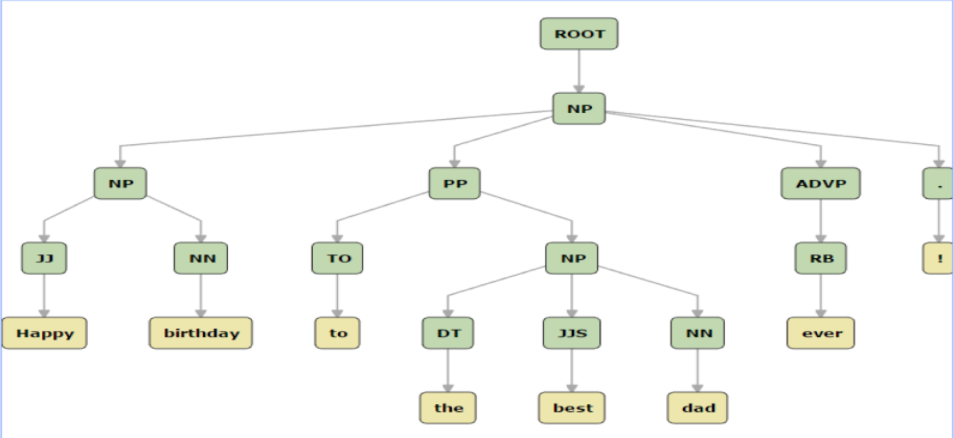
\includegraphics [width=\textwidth] {sf-parsetree.png}    
	\caption{A sample parse tree generated using Stanford CoreNLP}
	\label{fig:sf-parsetree}
\end{figure}

However, the above steps do not work in all cases. Given a sample post -- ``\textit{Happy Birthday to the best dad ever!}”, Stanford CoreNLP generates the parse tree shown in \figref{fig:sf-parsetree}, which contains the tokens, their POS tags and their dependencies. The object is ``\textit{best dad}”; however, the post does not contain any verbs. Posts with no verbs will have to rely on the event classification algorithm to determine its category, in this case, it is a \textit{celebrating} post because of the keyword ``birthday”.

The accuracy of the POS tagging also relies on Stanford CoreNLP, which led to problems because Stanford CoreNLP is not perfect. Depending on the punctuations, for example, a sentence's POS tagging changes. 

To illustrate, the post, ``Happy friendversary thesismate HAHAHA”, with a tagged person named ``Camille Saavedra,” shows up in the generated story as ``Robee celebrated friendversary thesismate HAHAHA with Camille”. This is because the POS tagger detected ``friendversary thesismate HAHAHA” as the main noun phrase in the post, and so considered it to be the object of the post. POS tagging can also change as a result of multilingual sentences; the use of mixed languages mess up the syntactic structure of the post, making it difficult for the parser to properly perform POS tagging.

After breaking down the sentence and completing the story plan, it is possible to have multiple words in the sentences which leads to the post possibly being classified into multiple types. For example, the sentence, ``Walking while eating gelato,” contains keywords for both \textit{travelling} and eating types of posts.

In the first iterations of the system, the post classification algorithm simply used co-location in order to check which types the post fell under. If it happened to have keywords for different types, the same sentence would appear multiple times in the generated story.

The post classification algorithm was changed: the keywords list was augmented with phrases from WordNet and ConceptNet; a scoring system has been implemented; and multiple post types are no longer possible. This change is further expanded on in Section 5.2, ``Event Classification.”

\subsection{Other Identified Characters}
\textit{Includes: Detecting rumors, contradictory information, sarcasms and humor, onomatopoeia, colloquial language}

Aside from the aforementioned characteristics of social media data, there are plenty of other characteristics relevant to this field. The first is that a lot of information posted online is speculative and wishful. Being able to detect rumors and distinguish them from facts is therefore necessary; however, it is not part of this research. Another characteristic of many posts is humor and/or sarcasm; being able to detect sarcasm and humor is a concern of empathic computing and human-computer interaction, and is not part of this research. Both of these characteristics can affect event detection (because, for example, a sarcastic post can be misconstrued by a computer as fact), and they become more relevant in the future as the topic expands, due to the need to accurately portray users' lives. Humor and hearsay can be misconstrued by the computer as fact, and therefore, wrong information can be generated.

Other characteristics which are a result of informality on social media include onomatopoeia and colloquial language. Onomatopoeia is the formation of a word from the imitation of a sound associated with it (e.g. ``oink oink”, ``buzz”, or ``haha”). For this research, laughter is removed as part of preprocessing; however, other onomatopoeic sounds are not preprocessed. Colloquial language refers to the use of very informal terms that are not standard; for example, texting in abbreviations (e.g. ``c u l8r”). For the purposes of this research, such language was not taken into consideration.


%section~~~~~~~~~~~~~~~~~~~~~~~~~~~~~~~~~~~~~~~~~~~~~~~~~~~~~~~~~~~~~~
\section{Event Classification}
Although Facebook's predefined activities feature is designed to enable users to easily classify their individual posts according to content, there are currently no available tools that can support the extraction of relevant elements from posts that use this feature. Furthermore, most Facebook users still prefer the traditional methods when crafting a post, i.e., typing text, and optionally combining photos and videos.

Given this limitation, available tools were used for gathering posts from an individual user's Facebook account, preprocessing the posts, classifying posts according to their event types, and then extracting event details.

\subsection{Keywords (Handcrafted)}
During data gathering, the initial dataset containing 2,514 posts were collected from 16 Facebook users. These posts were manually classified based on what the researchers think was the correct classification. It is important to note that at first, there were 15 types of posts, each with their own co-locating words; later on, it was then trimmed down to four categories of posts. These categories were chosen based on the frequency count of the posts classified to be as events. These categories were: \textit{celebrating, travelling, eating,} and \textit{drinking}. Posts classified under these categories were analyzed and a reference table (shown in \ref{tab:EventClassification}) containing the predefined keywords commonly associated with each event category was derived. Other posts not classified under these categories and no event posts were disregarded.

\clearpage
\begin{table}[ph!]   %t means place on top, replace with b if you want to place at the bottom
	\centering
	\caption{Classification of Facebook Posts based on Keywords} \vspace{0.25em}
	\begin{tabular}{|p{1.5in}|p{2in}|} \hline
		\centering Type of Post & Co-Locating Words \\ \hline
		Celebrating & 
			 Birthday \\
			 &  Celebrate \\
		 	&Congratulations \\
			 & Congrats \\
			 & God bless \\		
			 & Bless \\
			 & Wish \\
			 & Happy \\
			 & Merry \\
			 & Party \\
		 \hline
		Traveling & 
			 Go \\ 
			 &  Travel \\ 
			 &  At \\
			 &  Visit \\
			 &  Drive \\
			 &  Road \\
			 &  Place \\
			 &  Far \\
			 &  Run \\
			 &  Walk \\
			 &  Adventure \\
			  & Bucket list \\
		 \hline
		Eating & 
			 Cook \\
			 &  Eat \\
			 &  Dine \\
			 &  Breakfast \\
			 &  Lunch \\ 
			 &  Dinner \\
			 &  Chicken \\
			 &  Burger \\
			 &  Grill \\
			 &  Bake \\ 
			 &  Fry \\
		 \hline
	\end{tabular}
	\label{tab:EventClassification}
\end{table}

Only posts under the four categories were analyzed to derive the keywords. For \textit{celebrating} events, words which usually indicate special events such as \textit{birthdays} and \textit{Christmas} are used. For posts on \textit{travelling}, synonyms as well as methods of traveling are used. For \textit{eating}, aside from synonyms, the meals of the day are also used as indicators.

Since the dataset derived from manual inspection is by no means exhaustive of all Facebook user accounts, the list of keywords is not complete, and needed to be expanded to improve the classification process. 

\subsection{Keywords from Existing Resources (ConceptNet and WordNet)}
In order to address the issue of lack of keywords, the combination of the outputs of the two lexical resources, WordNet and ConceptNet, were used to populate the keywords list to be used later for event classification (as shown in \ref{tab:EventClassificationWordNet} and \ref{tab:EventClassificationConceptNet}). 

Initially, the plan was only to use WordNet only by extracting related concepts through its related senses. However, the lexical knowledge contained in WordNet was found to be insufficient for our purpose, as many terms (specifically physical objects) do not exist in it. To increase the coverage, ConceptNet's lexical and semantic knowledge was utilized to derive related contexts in which the words \textit{celebrating}, \textit{travelling}, \textit{eating}, and \textit{drinking} are found. Specifically, semantic relations such as ``IsA”, ``MadeOf” were used to derive the concepts. Table \ref{tab:SemanticsDescription} shows the complete list of relations used and their descriptions.  ConceptNet also contained a very minimal amount of Filipino words; these were also extracted to handle posts that contain Filipino words. An example Filipino word, \textit{paglalakbay}, is shown in \ref{tab:EventClassificationConceptNet} as one of the keywords for the \textit{travelling} post.

\clearpage
\begin{table}[ph!]   %t means place on top, replace with b if you want to place at the bottom
	\centering
	\caption{List of semantic relations and their descriptions} \vspace{0.25em}
	\begin{tabular}{|p{1.5in}|p{2in}|} \hline
		\centering Relationt & Description\\ \hline
		HasFirstSubevent & What do you do first to accomplish it? \\ \hline
		HasLastSubevent & What do you do last to accomplish it? \\ \hline
		HasPrerequisite & What do you need to do first? \\ \hline
		MadeOf & What is it made of? \\ \hline
		IsA & What kind of thing is it? \\ \hline
		AtLocation & Where would you find it? \\ \hline
		UsedFor & What do you use it for? \\ \hline
		CapableOf & What can it do? \\ \hline
		MotivatedByGoal & Why would you do it? \\ \hline
		Desires & What does it want? \\ \hline
		DefinedAs & How do you define it? \\ \hline
		InstanceOf & What type of thing is it a specific example of? \\ \hline
		CausesDesire & What does it make you want to do? \\ \hline
		Causes & What does it make happen? \\ \hline
		HasSubevent & What do you do to accomplish it? \\ \hline
		HasProperty & What properties does it have? \\ \hline
		PartOf & What is it part of? \\ \hline
		ReceivesAction & What can you do to it? \\ \hline
		CreatedBy & How do you bring it into existence? \\ \hline
	\end{tabular}
	\label{tab:SemanticsDescription}
\end{table}
\clearpage
\begin{table}[ph!]   %t means place on top, replace with b if you want to place at the bottom
	\centering
	\caption{Keywords Derived from ConceptNet (see Appendix \ref{sec:appendixl} for full list)} \vspace{0.25em}
	\begin{tabular}{|p{1.5in}|p{2in}|} \hline
		\centering Type of Post & Co-Locating Words \\ \hline
		Celebrating 
		& Victory \\ 
		& Christmas \\ 
		& Firework \\ 
		& Birthday \\ 
		& Toast \\\hline
		Eating  
		& Chew \\ 
		& Swallow \\ 
		& Food \\ 
		& Cook \\ 
		& Plate \\ 
		& Kain \\\hline
		
		Drinking 
		& Thirsty \\ 
		& Liquid \\
		& Bottle \\ 
		& Beer \\ 
		& Lemonade \\ 
		& Inumin \\\hline
		Traveling 
		& Passport \\ 
		& Fun \\ 
		& Explore \\ 
		& Pack \\ 
		& Adventure \\ 
		& Paglalakbay  \\\hline
	\end{tabular}
	\label{tab:EventClassificationConceptNet}
\end{table}

\clearpage
\begin{table}[ph!]   %t means place on top, replace with b if you want to place at the bottom
	\centering
	\caption{Keywords Derived from WordNet (see Appendix X for full list \ref{sec:appendixl})} \vspace{0.25em}
	\begin{tabular}{|p{1.5in}|p{2in}|} \hline
		\centering Type of Post & Co-Locating Words \\ \hline
		Celebrating 
			& Celebrate \\
			& Observe\\
			& Fete\\
			& Lionize
		\\ \hline
		Eating 
			& Eat\\
			& Feed\\
			& Depletion\\
			& Consume 
		 \\ \hline
		Drinking 
			& Booze\\
			& Salutation\\
			& Pledge\\
			& Salute\\
			& Toast
		 \\ \hline
		Traveling
			& Movement\\
			& Traveler\\
			& Locomotion\\
			& Journey\\
			& Trip\\\hline
	\end{tabular}
	\label{tab:EventClassificationWordNet}
\end{table}
\clearpage
\begin{table}[ph!]   %t means place on top, replace with b if you want to place at the bottom
	\centering
	\caption{Keywords Derived from ConceptNet (see Appendix \ref{sec:appendixl} for full list)} \vspace{0.25em}
	\begin{tabular}{|p{1.5in}|p{2in}|} \hline
		\centering Type of Post & Co-Locating Words \\ \hline
		Celebrating 
			& Victory \\ 
			& Christmas \\ 
			& Firework \\ 
			& Birthday \\ 
			& Toast \\\hline
		Eating  
			& Chew \\ 
			& Swallow \\ 
			& Food \\ 
			& Cook \\ 
			& Plate \\ 
			& Kain \\\hline

		Drinking 
			& Thirsty \\ 
			& Liquid \\
			& Bottle \\ 
			& Beer \\ 
			& Lemonade \\ 
			& Inumin \\\hline
		Traveling 
			& Passport \\ 
			& Fun \\ 
			& Explore \\ 
			& Pack \\ 
			& Adventure \\ 
			& Paglalakbay  \\\hline
	\end{tabular}
	\label{tab:EventClassificationConceptNet}
\end{table}

After integrating WordNet and ConceptNet, the system has 1,697 co-locating words across all event types. Table \ref{tab:Co-locatingWords} shows a breakdown of the co-locating words.
\begin{table}[ph!]   %t means place on top, replace with b if you want to place at the bottom
	\centering
	\caption{Number of the co-locating words per event type and source} \vspace{0.25em}
	\begin{tabular}{|p{1in}|c|c|c|} \hline
		\centering Event Types & from WordNet & from ConceptNet & TOTAL \\ \hline
		Celebrating & 9 & 350 & 359 \\ \hline
		Eating & 17 & 400 & 417 \\ \hline
		Drinking & 24 & 492 & 516 \\ \hline
		Traveling & 16 & 389 & 405 \\ \hline
		TOTAL & 66 & 1631 & 1697 \\ \hline
	\end{tabular}
	\label{tab:Co-locatingWords}
\end{table}

Initial testing was done to the keywords from ConceptNet and WordNet. However, the results were low due to the fact that the list of keywords were both broad and vague. The list contains 1,697 keywords including repeating words that may overlap from one category to the other. When the classifier encountered this problem, it immediately classify this to the first category according to the hierarchy to be explained in Section 5.3.4 - Scoring System which may lead to misclassification. Words that are not closely related to the category were also included that causes the system to classify a post under that category when it should not be the case. Thus, the keyword list needs to be pruned hoping to attain a better result. Analysis was done to determine which keywords need to be removed. Removing excess keywords limits the outliers (keywords far in relation to the category) from affecting the classification of the posts. This concentrates the keywords to the words with the closest relation to the categories, thus improving the classification.

\subsection{Pruned Keywords}
Removing the excess keywords limits the outliers (or the keywords far in relation to the category) from affecting the classification of the posts. This concentrates the keywords to the words with the closest relation to the categories, thus improving the classification.

The set of derived keywords were pruned manually following a set of rules:
\begin{itemize}
	\item Rules to retain a keyword:
	\begin{itemize}
		\item 	One word verbs relating to the category which may or may not be followed by a noun (i.e. chew, swallow, eat meal in eating category; drink coffee,thirst, hydrate for drinking category; throw party for \textit{celebrating} category; take bus, fly airplane and go sightseeing for \textit{travelling} category)
		\item Proper nouns pertaining to the action (i.e. coffee, tea, lemonade in drinking category, cookie and meal in eating category; cheer )
		\item Modes of transportation, experience and verbs indicating travelling (i.e. take airplane, drive road, sightsee, jet lag for travelling)
		\item Special events and holidays that may or may not come as greetings (i.e. anniversary, friendversary, Merry Christmas, Christmas Eve, New Year, wedding, party)
	\end{itemize}
	\item Rules to remove a keyword:
	\begin{itemize}
		\item Articles (i.e. a, an, the)
		\item Common verbs (i.e. get, become and go) 
		\item Repeating words (i.e. eat , cookie, eat cookie; remove eat cookie)
		\item Words that have no connection to the categories (i.e. esophagus, dance, call family, wet mouth, pee, fridge)
		\item Overlapping category (i.e. 'Champagne’ which is included both in drinking and celebrating; would be removed in celebrating since the action weighs more on drinking.)
	\end{itemize}
\end{itemize}

After the pruning process, the system now has 521 co-locating words across all event types. Table \ref{tab:pruning-results} shows a breakdown of the co-locating words.
\begin{table}[ph!]   %t means place on top, replace with b if you want to place at the bottom
	\centering
	\caption{Number of the co-locating words per event type and source after pruning process} \vspace{0.25em}
	\begin{tabular}{|p{1in}|c|c|c|} \hline
		\centering Event Types & from WordNet & from ConceptNet & TOTAL \\ \hline
		Celebrating & 9 & 67 & 76 \\ \hline
		Eating & 17 & 108 & 125 \\ \hline
		Drinking & 24 & 197 & 221 \\ \hline
		Traveling & 16 & 83 & 99 \\ \hline
		TOTAL & 66 & 455 & 521 \\ \hline
	\end{tabular}
	\label{tab:pruning-result}
\end{table}

\subsection{Naive-based System}
The initial post classification algorithm used the handcrafted keywords list to classify the posts. The algorithm of the first implementation was:
\begin{lstlisting}
	For each token in the sentence:
		For each keyword:
			If token matches keyword:
				Get keyword category
				Set category as post type
\end{lstlisting}

However, several issues were encountered. First, consider the post ``Eating and drinking at McDo.”, the initial classifier would classify this post as both eating and drinking post. Later on, when generating the story, it will contain redundant sentences. Another issue found was that the classifier is very sensitive. For example, the post ``At your service”, was classified as a travelling post because of the keyword “at”. Because of this, the classification algorithm was improved to cater these issues.

\subsection{Scoring System}
As stated in 5.1.3, posts are classified by their relevant keywords. This is done by first breaking down the post into its individual sentences and getting the part-of-speech tags of each token, which is handled by Stanford CoreNLP. Afterwards, the verbs are lemmatized, and all relevant tokens in the sentence are cross-referenced with the table of classification stated in 5.2.1.

Because a single sentence can contain multiple verbs or words signifying events, the first iteration of the automated classifier classified this into multiple event categories. For example, the sentence, ``\textit{Walking around the streets of Rome while eating delicious gelato,}” was classified as an eating event and a travelling event. 

To avoid redundancy and the loss of context in downstream tasks, the classification algorithm has been revised to use a scoring system, and the sentence is assigned the category with the highest score. If multiple event categories bear the same score, a bias scheme based on the hierarchy of \textit{celebrating} =$>$ \textit{eating} =$>$ \textit{drinking} =$>$ \textit{travelling} will be followed. The hierarchy was based on the frequency count of the classified events using the gathered posts. A threshold value of 2 was also set to minimize the occurrence of misclassification. The threshold was set to 2 because the most common keywords contained at least two words. Most classified posts contain keywords such as ``drink coffee”, ``eat food”, ``Happy Birthday”, and ``Merry Christmas”. Setting the threshold to 1 increases the likelihood to be misclassified such as the previous example ``At your service”. However, increasing the threshold to 3 would then be limiting most of the posts. This would then result to under classification which means the value of false negative would increase.

Consider the sentence, ``\textit{I'd love to take a walk on the park someday.}” The presence of the word walk in the list of keywords led the no-score classifier to consider this sentence as a travelling event, when it should not have been the case. In the score-based classifier, only sentences such as ``\textit{I'm going on an adventure to check off one from the bucket list}”, which has a score of 3 because of the words ``\textit{going}”, ``\textit{adventure}”, and ``\textit{bucket list}	” and thus, was categorized as a \textit{travelling} event.

The initial algorithm for the score-based classifier was:
\begin{lstlisting}
	Set initial score to 0 for each category
	For each token in the sentence:
		For each keyword:
			If token matches keyword
				Get keyword category
				Increment score
	Set category with highest score as post type
\end{lstlisting}

But this new scoring algorithm still poses some issues. Using the example ``At your service.”, the classifier matched the keyword ``at” so the category travelling has 1 point. The keywords for other categories no not match any of the words, so the highest score was \textit{travelling}. But the example post is not a \textit{travelling} post, thus, the algorithm was tweaked to fix issues like this. The latest algorithm needs to satisfy at least 2 points for it to be classified as that category. The final algorithm was:
\begin{lstlisting}
	Set initial score to 0 for each category
	For each token in the sentence:
		For each keyword:
			If token matches keyword
				Get keyword category
				Increment score
	If category with highest score >= threshold
		Set category with highest score as post type
\end{lstlisting}

%section~~~~~~~~~~~~~~~~~~~~~~~~~~~~~~~~~~~~~~~~~~~~~~~~~~~~~~~~~~~~~~
\section{Life Story Generation}
The text generation module is responsible for generating the appropriate story segments that make up the entire life story generated by the system. There are three components of the text generation module, namely the GenIntro, GenBody, and GenConclusion. GenIntro is the module applied to the data determined to be “facts” or direct knowledge, such as family and work information; GenBody is applied to generate the body of the life story from the data processed in the Data Processing module; and GenConclusion is the module applied to the data determined to be “facts” or direct knowledge.

Following the NLG pipeline of Reiter \& Dale (1997; 2000), story generation usually proceeds in three main steps, namely content determination, discourse planning, and surface realization. Initially, the system used a template-based generation algorithm, but later switched to a grammar-based (or script-based; the two terms are interchangeable in the context of our research) algorithm. A thorough discussion of the rationale behind the switch is explained in Section 5.3.6 Switching to Grammar-Based Generation.

\subsection{Template-Based Generation}
Following the NLG pipeline mentioned earlier, content determination for GenIntro and the GenConclusion involve deriving data supplied by the user themselves. The system initially used templates and was therefore \textit{template-based}. The algorithm for GenIntro is as follows:
\begin{lstlisting}
	For each subtemplate:
		Get all possible templates based on the available data
		Randomly choose 1 template
		Fill the template with the correct data
	Connect all phrases to form the whole introduction
\end{lstlisting}

For example, when generating the introduction, the system follows a general template of:
\begin{itemize}
	\item $<$NAME$>$ $<$\textit{intro\_birth}$>$  $<$\textit{intro\_education\_gs}$>$ $<$\textit{intro\_education\_gs}$>$ $<$\textit{intro\_education\_college}$>$ $<$\textit{intro\_work}$>$ $<$\textit{location, hometown}$>$ $<$\textit{intro_family}$>$
\end{itemize}

Then, each of these has their own sub-templates. For instance, $<$\textit{intro\_birthday}$>$ can choose from the following templates:
\begin{itemize}
	\item $<$\textit{intro\_birth\_circumstance}$>$
	\item Is a $<$AGE$>$-year old $<$GENDER$>$ who
\end{itemize}

Then, the $<$\textit{intro\_birth\_circumstance}$>$ can still be broken down to other sub-templates such as:
\begin{itemize}
	\item , born on $<$BIRTHDAY$>$,
	\item was born on $<$BIRTHDAY$>$
\end{itemize}

Finally, upon choosing the templates at random, the system would then fill in the blanks with the data stored in the \textit{direct knowledge} table as follows:

\begin{center} Robee, is a 21-year old female who has yet to get her college diploma from De La Salle University. \end{center}

While for the GenConclusion (Liked pages), the general template was: $<$NAME$>$ likes $<$liked pages$>$ and the algorithm is as follows:
\begin{lstlisting}
	For each category:
		Use the template: <category> such as <pages>
		In generating the <pages> phrase:
			Check how many examples from that category.
			If yes, iterate through each one of them. Use ``,” to connect the first 2 then use ``and” to connect the last. Get the plural form of the category.
			If only 1, no need to determine connector. And no need to get plural form of the category.
	Replace <pages> to the generated phrase
	Replace <liked pages> to the generated phrase
\end{lstlisting}

Lastly, for the GenConclusion (Attending Events), it uses the general template: <NAME> attended <events> and the algorithm is as follows:

\begin{lstlisting}
For each event:
Use the template: <event name> at <location>
In generating the <events> phrase:
Check how many events
If more than 1, iterate through each and one of them. Use “,” to connect the first few events then use “and” to connect the last. Check if there is a location for each event.
Replace <events> to the generated phrase
\end{lstlisting}

Same algorithm was used in the GenConclusion - Interested Events but this time is uses the general template: $<$NAME$>$ was interested in attending events such as $<$events$>$.

The system would then chain templates like these together in order to create the introductory and conclusion paragraphs. Following the NLG pipeline mentioned earlier, this would be discourse planning, but very minimal discourse planning is performed in a template-based approach due to how simple it is.  Each time, it would have to choose a sentence at random. This poses a problem: the templates are manually created by a person, and so if a new sentence type were to be implemented, such as about a person's phone number, a template would have to be created, which includes all possible varieties of sentences that can be formed which talk about the phone number. Also, note that since templates are not flexible, it introduces problem for surface realization: there are usually grammar problems encountered such as the use of the correct pronoun or the correct preposition. These would then have to be worked around by the system, which means more work had to be done.

Therefore, a way to dynamically generate sentences using NLG is needed for extensibility and scalability. Works such as (\cite{chen2008natural}; \cite{sleimi2016generating}) have shown the power of using RDF data to construct descriptive sentences dynamically. This approach was adapted, which enabled support for graph-based, or grammar-based, text generation, using scripts instead of templates. 

This meant that the story planning and the surface realization parts are changed, since the content determination stays the same.

\subsection{Scripts}
The story generator uses Resource Description Framework (RDF) data to construct sentences, with the help of SimpleNLG. RDF data consists of (\textit{subject-predicate-object}) triples such as (\textit{Robee, nationality, Taiwanese}). The subject indicates the resource, while the predicate indicates the trait or aspect of the resource which also shows the relationship between the subject and the object. As illustrated in \figref{fig:rdf}, RDF data can be represented by a graph in which edges are labelled with properties and vertices with subject and object resources.

\begin{figure}[!htb]
	\centering           
	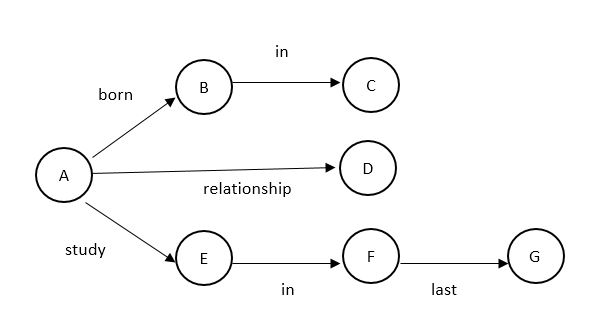
\includegraphics  [width=4.5in,height=4.2in,keepaspectratio] {graph-rdf.jpg}    
	\caption{An example of a graph representation of RDF data. (A, birthPlace, F) is connected to (F, country, H), for example. }
	\label{fig:rdf}
\end{figure}

Each vertex in the graph is an object (not to be confused with \textit{direct object}), and for the purposes of story generation, each object is described in a sentence (turning it into an assertion or a message). Aside from the name of the object, assertions can be a combination of the following.

For the introduction, the assertions are:
\begin{itemize}
	\item person (lastName, firstName, middleName)
	\item gender(obj)
	\item livingIn(obj)
	\item family(relationship, names$<$$>$)
	\item roleFam(obj)
	\item occupation(obj)
	\item birth(date, place)
	\item education(institution, type, yeargrad, course)
	\item work(institution, startDate, endDate, location)
\end{itemize}

And for the conclusion:
\begin{itemize}
	\item person (\textit{lastName, firstName, middleName})
	\item eventsGoing(\textit{name, location})
	\item eventInterested(\textit{name, location})
	\item likes(\textit{category, page$<$$>$})
\end{itemize}
These assertions are then filled with information from the user data, such that, for example,

\begin{center} person (lastName, firstName, middleName) \end{center}

becomes

\begin{center} person (Hade, Alden Luc, Rosqueta) \end{center}

A set of story grammar rules were used to form English sentences. Section 5.4.6, Switching to Grammar-Based Generation, discusses the reasons why the implementation of the Introduction and Conclusion shifted from Template-Based Generation to Grammar-Based Generation. This will be evident later when we discuss the evolution from templates to grammars in generating the Introduction (5.4.3), Conclusion (5.4.4), and Body (5.4.5).

The grammar rules used for the introduction are shown in \ref{tab:GrammarRules}; (\ref{tab:GrammarRules} is shown here as an example; the grammar rules for the conclusion and body are in their respective sections later on.)

\begin{table}[ph!]   %t means place on top, replace with b if you want to place at the bottom
	\centering
	\caption{Grammar Rules Used for the Introductory Paragraphs} \vspace{0.25em}
	\begin{tabular}{|p{2in}|p{2.5in}|} \hline
		$<$INTRODUCTION$>$ &$<$SENTENCE$>$+ \\ \hline
		$<$SENTENCE$>$ & $<$subject$>$ $<$PREDICATE$>$ \\ \hline
		$<$PREDICATE$>$ & $<$verb$>$ $<$OBJECT$>$ \\ \hline
		$<$OBJECT$>$ & $<$noun$>$ [$<$preposition phrase$>$*] $|$$|$ \newline
		$<$article$>$ $<$noun$>$ [$<$preposition phrase$>$*] $|$$|$\newline
		$<$preposition phrase$>$ \\ \hline
	\end{tabular}
	\label{tab:GrammarRules}
\end{table}
The system reads the grammar file using the bottom up approach, where it will start with filling the grammar rules at the bottom with data, before working its way up. Grammar rules that have not been filled up will be removed, while grammar rules that have been filled will be used to generate the assertion. The system then loops through the list of assertions for the introduction and conclusion, fills them with data, generates the sentences with the help of the grammar rules, and puts the sentences together, in order to generate the paragraphs for the introduction and conclusion respectively. 

An example for the introduction would be that the following assertions

\begin{center} person (lastName, firstName, middleName) \end{center}
\begin{center} gender(gender) \end{center}
\begin{center} livingIn(location) \end{center}

with the help of data from Facebook would become

\begin{center} person (``Te'', ``Robee Khyra'', ``'') \end{center}
\begin{center} gender(``Female'') \end{center}
\begin{center} livingIn(``Manila, Philippines'') \end{center}

and would generate the following RDF triples (note that the surface form of the verbs are defined as part of the RDF triples):

\begin{center} (``Robee Khyra Te'' ``is'' ``female'') \end{center}
\begin{center} (``Robee Khyra Te'' ``lives in'' ``Manila, Philippines'') \end{center}

Each of these RDF would then become a sentence of the form

\begin{center} $<$sentence$>$	-$>$	$<$subject$>$ $<$predicate$>$ \end{center}

where

\begin{center} $<$predicate$>$	-$>$	$<$verb$>$ $<$object$>$ \end{center}

Therefore, the generated sentences would become

\begin{center} Robee Khyra Te is female. \end{center}
\begin{center} Robee Khyra Te lives in Manila, Philippines. \end{center}

Putting the sentences next to each other would result in a paragraph. 

\subsection{Generating the Introduction}
The introduction paragraphs are meant to present the Facebook user to the reader, to provide a background of the subject as if in a real biography. 

\underline{\textbf{Template-Based Generation Iteration 1}} \newline
The very first iteration of the generation of introduction was done simply to check whether the data is being used correctly, and how well the templates would look when put together into a paragraph. The templates were simply filled up and concatenated with each other. Since each template was not a complete sentence by itself but rather a clause, the output paragraph was not separated into sentences. Also, templates which were not filled with data would glaringly have missing information. An example of this is shown below.

\begin{center} Robee Khyra Te was born \underline{\textbf{on 05/25/1996 got her high school diploma}} from Chiang Kai Shek College \underline{\textbf{in 2013 graduated college}}  in De La Salle University \underline{\textbf{last 0 worked from}} 2013-09-01 to 2014-04-30 at University Student Government, \underline{\textbf{DLSU is from $<$hometown$>$}} she is the daughter of Ian Quintin and Katherine Ann Te.
 \end{center}

\underline{\textbf{Template-Based Generation Iteration 2 - Missing Information}} \newline
For the first true iteration of GenIntro, these templates were put together into sentences with the help of SimpleNLG. However, it still could not account for missing information:

\begin{center} Robee Khyra Te was born on 05/25/1996. \underline{\textbf{She got his high school}} diploma from Chiang Kai Shek College in 2013. \underline{\textbf{She got his college diploma from De La Salle University on $<$grad\_year$>$.}} She worked from \underline{\textbf{2013-09-01 to 2014-04-30}} at University Student Government, DLSU. She hailed from Manila, Philippines, and is now living in Manila, Philippines. \underline{\textbf{She she}} is the daughter of Ian Quintin and Katherine Ann Te.
 \end{center}

Worth noting is that the template in the database, since it was created by a human, assumed a lot of things about what the computer can do by itself (such as the simple issue of separating the paragraph into sentences, or determining the user's gender). 

For the next iterations, the missing information were accounted for. If a template cannot be filled completely, clauses related to the missing information (such as the dependent clause ``from $<$hometown$>$”) are removed. The introduction text also still did not know if a student has graduated already or is still studying, for example. Also, the gender of the subject was not yet determined, so there are contradicting pronouns in the paragraph.

\underline{\textbf{\underline{\textbf{Template-Based Generation Iteration 2 - Missing Information}} \newline}} \newline
However, the text was still not completely readable. Dates were listed as they are in the database rather than written like natural language. And so, the generation was further improved. The gender of the user was eventually determined correctly; dates were made readable; and the system now took into account the years of education or work in order to determine whether they happened in the past or not, and then explain them in a way that makes sense. Another problem was redundant data: if the current city and hometown are the same, the same town appeared twice, perhaps even in the same sentence.

The last iteration before switching to grammar-based story generation produced an introduction which provides a concise, coherent, and grammatically-correct description of basic information about the subject's life.

\begin{center} Robee Khyra Te, born on \underline{\textbf{May 25, 1996}}, got her \underline{\textbf{high school diploma}} from Chiang Kai Shek College \underline{\textbf{last 2013}}. She \underline{\textbf{has yet to get}} her college diploma from De La Salle University. She worked from \underline{\textbf{September 01, 2013 to April 30, 2014}} at University Student Government, DLSU. \underline{\textbf{She is from Manila, Philippines.}} She is the daughter of Ian Quintin and Katherine Ann Te. \end{center}

The grammar rules for the grammar-based story generation of the introductions are shown in \ref{tab:GrammarRules}.

\begin{center} Robee Khyra Te , born on May 25, 1996 , got her high school diploma from Chiang Kai Shek College last 2013. She has yet to get her college diploma from De La Salle University. She worked from September 01 , 2013 to April 30 , 2014 at University Student Government, DLSU. She is from Manila, Philippines. She is the daughter of Ian Quintin and Katherine Ann Te.
\end{center}

\underline{\textbf{Grammar-Based Generation Final Output}} \newline

\subsection{Generating the Conclusion}
The conclusion is meant to summarize what was said about the user in the body of the life story by stating their likes. These likes are supported by giving examples of related Facebook pages that the user has Liked. But the conclusion also provides support to these likes by showing examples of events attended by the person.

\underline{\textbf{Template-Based Generation Iteration 1}} \newline
The very first iteration of the generation of conclusion was done simply to list down the pages that the user likes per category in a form of a paragraph. An example of this is shown below.

\begin{center} Robee Khyra Te likes Community such as Technology Impact Summit 2017, RVR COB Week 2017, Annyeong Oppa , Romance of the Three Kingdoms, Status: Speak Up, Oms Giving, The Border Collective, University Vision - Mission Week 2016, DLSU Hackercup 2015, Handog 2015, Jazzy's Accessories, DLSU - Manila Secret Files, SOLIDarity Against Abuse, Alive: Touch the Sky, Hero of D Day UP, CCS Month 2014: Conexus, CRYO, L E G A C Y, KPOP Concert Philippines, DLSU Administration, CSO Annual Recruitment Week 2014, LPEP 2K14, Sweetooth , Sims 4 and Millennia: Ignite the Revolution . Robee Khyra Te likes Artist such as Calleftgraphy , Park Shin Hye - PSH ë ° ? ì ? í??, Song Hye Kyo , Song Joong Ki ì ?¡ ì¤ ?ê ¸ ° , Daehan Minguk Manse, Ha Ji Won (í?? ì § ? ì ??), Nikki Co, Lee Sang Yoon - Turkey, Daniel John Ford E. Padilla, Ji Sung ì § ? ì ? ± - ã??ã?½ã?³ - æ ± å ??, JYP Actors, Lee Bo Young, Kim Woo Bin, Jo Seung Woo ì ¡° ì ? ¹ì ? ° , Lee Jong Suk ì ? ´ì ¢? ì ??, Lee Min Ho's World, Lee Minho ( ì ? ´ ë ¯ ¼í? ¸ ), Lee Bo Young / ì ? ´ ë³ ´ì ?? and Lee Bo - young
\end{center}

\underline{\textbf{Template-Based Generation Iteration 2 - Limiting the list}} \newline
The initial output did not have any limit as to how long it would be, and so all of the user’s likes and the events they attended were slammed into the paragraph. This was quickly corrected by limiting the conclusion paragraph(s) to three Liked pages per type.

\begin{center} Robee Khyra Te likes \underline{\textbf{Community}} such as Technology Impact Summit 2017, RVR COB Week 2017, \underline{\textbf{A}}nnyeong Oppa. \newline
	\underline{\textbf{Robee Khyra Te likes Artist}} such as Calleftgraphy, Park Shin Hye-PSH ë°?ì? í??\underline{\textbf{, S}}ong Hye Kyo. \newline
	\underline{\textbf{Robee Khyra Te likes TV Show}} such as Cinderella and Four Knights, Moonlight Drawn by Clouds - Korean Drama, \underline{\textbf{D}}escendants of the Sun. \end{center}

\underline{\textbf{Template-Based Generation Iteration 3 - Forms, Punctuation and Capitalization}} \newline
The problems dealt with in the improvement of the conclusion paragraph(s) were all related to grammar and punctuation and capitalization errors. However, first, there was the need to teach the generator to use pronouns, because saying the full name in each sentence is redundant. Some of the simple sentences to form longer sentences were then combined, once the system was taught to use pronouns:

\begin{center} Robee Khyra Te \underline{\textbf{likes Communities}} such as Technology Impact Summit 2017, RVR COB Week 2017 \underline{\textbf{, A}}nnyeong Oppa \underline{\textbf{., Artists}} such as Calleftgraphy, Park Shin Hye-PSH ë°?ì? í??\underline{\textbf{, S}}ong Hye Kyo\underline{\textbf{., TV Shows}} such as Cinderella and Four Knights, Moonlight Drawn by Clouds - Korean Drama\underline{\textbf{, D}}escendants of the Sun. \end{center}

Also, a problem with the category of the pages is evident. Notice that even though there are three examples to support a single category, the category name used was still written in its singular form. The initial algorithm for this was to create a manual surface realizer to correct the form of the category.
\begin{lstlisting}
if( lastLetter is ‘y’)
	Change last letter to “ies”;
Else if(lastLetter is ‘s’)
	Append “es”;
Else
	Append “s”;
\end{lstlisting}

However, in the latter part of the development, the developers utilizes SimpleNLG for getting the plural form of the category. 

Finally, the events attended by the user were plugged into the conclusion.

 \clearpage
\begin{table}[ph!]   %t means place on top, replace with b if you want to place at the bottom
	\centering
	\caption{Grammar Rules Used for the Conclusion Paragraphs} \vspace{0.25em}
	\begin{tabular}{|p{2in}|p{2.5in}|} \hline
		$<$CONCLUSION$>$ & $<$SENTENCE$>$+ \\ \hline
		$<$SENTENCE$>$ & $<$subject$>$ $<$verb$>$ $<$PHRASES$>$ \\ \hline
		$<$PHRASES$>$ & $<$SIMPLE\_PHRASE$>$ $|$$|$ \newline $<$COMPLEX\_PHRASE$>$ \\ \hline
		$<$SIMPLE\_PHRASE$>$ & $<$NOUN\_PHRASE$>$+ \\ \hline
		$<$NOUN\_PHRASE$>$ & $<$noun$>$ $<$LIST$>$ \\ \hline
		$<$LIST$>$ & ``such as” ($<$noun$>$ [$<$prepositional phrase$>$*])+ \\ \hline
		$<$COMPLEX\_PHRASE$>$ & $<$GERUND\_PHRASE$>$ $<$INFINITIVE\_PHRASE$>$ $<$LIST$>$ \\ \hline
		$<$GERUND\_PHRASE$>$ & in $<$verb$>$ \\ \hline
		$<$INFINITIVE\_PHRASE$>$ & to $<$noun$>$ \\ \hline
	\end{tabular}
	\label{tab:GrammarRules-Conclusion}
\end{table}

\underline{\textbf{Grammar-Based Generation Final Output}} \newline
\begin{center}
	Robee Khyra Te likes communities such as Technology Impact Summit 2017, RVR COB Week 2017, Annyeong Oppa, artists  such as Calleftgraphy, Park Shin Hye-PSH, Song Hye Kyo, TV shows  such as Cinderella and Four Knights, Moonlight Drawn by Clouds - Korean Drama, Descendants of the Sun.
	\newline
	Robee Khyra Te attended Cybersecurity and International Relations, Publication Writing Workshop, LSCS Christmas Party! at The Manila Residences Tower II in Manila, CCS Month 2016: Festivo at Henry Sy Bldg, De La Salle University - Manila and Technology Summit 2016 Forum at De La Salle University in Manila.
\end{center}

The grammar rules for the grammar-based generation approach for the conclusion paragraphs are shown in \ref{tab:GrammarRules}.

The outputs for grammar-based story generation for both introduction and conclusion are similar, with the most significant changes happening under the hood rather than on the surface (or the generated story, in this case).

\subsection{Generating the Body}
The body is meant to show events regarding \textit{celebrating, eating, drinking,} and \textit{travelling}, with the observation that these posts are most explicitly stated by Facebook users. The bulk of the work for the story generator is in producing the text for the body of the life story. Following the NLG pipeline mentioned earlier, content determination involves utilizing the events that were derived from processing and classifying the posts. Story planning is then responsible for organizing and sequencing the events into a coherent story plan, which is comprised of sequences of events of the form

\begin{center} Verb (doer, receiver of the action, object, date, location) \end{center}

In generating the story plan, the planner takes into consideration the temporal and the topical relations of events. Topical relations are used to generate paragraphs; one topic (or event category) equates to one paragraph. Within each paragraph, events are ordered based on their temporal relations, which are determined from the timestamps attached to each post and linked to the corresponding events.

Surface realization converts each verb entry in the story plan into a sentence to express the date(s) of occurrence, as well as the people and places involved in each event. The task involves defining the input specifications for each sentence to be generated. This includes setting the user and other people tagged as the actor or doer of the action, the particular action, the object, and the tense of the verb.

The algorithm used for generating the body paragraphs was:

\begin{lstlisting}
	Get all event posts
	Sort by category
	For each category:
		Sort by date
		For each post:
			Generate a sentence for it
		Add a summary sentence for each paragraph
\end{lstlisting}

The summary sentences for each categories were:
\begin{itemize}
	\item Celebrating - With whom did the user celebrated the most
	\item Eating/Drinking - Where have you eaten
	\item Travelling - Where have you been locally and internationally
\end{itemize}

\underline{\textbf{Grammar-Based Generation Iteration 1}} \newline
\begin{table}[ph!]   
	\centering
	\caption{Sample Facebook posts classified as \textit{celebrating} posts, along with their metadata} \vspace{0.25em}
	\begin{tabular}  {|p{2in}|p{1.5in}|p{1.5in}|}  \hline
    \multicolumn{1}{|c|}{Original Post} & \multicolumn{2}{c|}{Metadata}\\ \hline
	Happy 18th Angie! &  date created & 10/03/14 \\ \hline
	
	{Happy anniversary Jamie HAHA} &  {date created} &{02/07/17} \\\cline{2-1}
	& {user tagged} & {Jamie} \\\hline
	
	{Happy friendversary thesismate!} &  {date created} & {02/14/17} \\\cline{2-1}
	&  {user tagged} &{Cam} \\\hline
	
	{Party party!} &  {date created} & {08/16/16} \\\cline{2-2}
	&  {user tagged} & {Shane} \\\cline{2-2}
	&  {location} & {Manila, Philippines} \\\hline
	
	\end{tabular}
	\label{tab:GrammarRules-celeb}
\end{table}

Consider the Facebook posts including the extracted metadata shown in Table \ref{tab:GrammarRules-celeb}, all classified as celebrating. The corresponding story plan was:

\begin{center} celebrating(Mae, null, Angie, 10/03/14, null) \newline
	celebrating(Mae, null, Jamie, 02/07/17, null) \newline
	celebrating(Mae, null, thesismate, 02/14/17, null) \newline
	celebrating(Mae, null, null, 08/16/16, null) \end{center}

and the resulting story text was: 

\begin{center}Mae celebrated Angie. Mae celebrated thesismate with Cam. Mae celebrated with Shane in Manila, Philippines. Mae celebrated anniversary Jamie HAHA with Jamie. \end{center}

\underline{\textbf{Grammar-Based Generation: Iteration 2 - Added Date, Location, and Tagged Friends}} \newline
In the early iterations of GenBody, each event leads to one sentence of the form ``On <date>, <actor> celebrated <activity> with <friend>.” But before that, the dates, location, and tagged were not even mentioned at all, and the activities identified were almost always wrong.

The problems encountered with this approach stem mostly from difficulty in parsing posts that are mostly informal in nature. Some posts are parsed incorrectly, leading to the wrong activity being articulated. For example, in the last sentence above, the identified activity from the post is ``anniversary jamie”.

\begin{center} On October 03, 2014, Mae celebrated Angie. On February 14, 2017, Mae celebrated thesismate with Cam. On August 16, 2016, Mae celebrated with Shane in Manila, Philippines. On February 07, 2017, Mae celebrated Jamie HAHA with Jamie. \end{center}

\underline{\textbf{Grammar-Based Generation: Iteration 3 - Topic Sentence and Temporal Relations}} \newline
One solution to improve the coherency and reduce the redundancy in the generated text is to take advantage of the temporal relations among events by sorting them from most recent to oldest according to their timestamp. This task is handled by the story planner. The surface realizer then applies aggregation to group related events together, i.e., those with closer temporal relations or those with the same people involved. Closer temporal relations mean either the same date, the same month or the same year.

\begin{center}Mae has celebrated most with Shane, Jamie and Cam. They celebrate together. A year ago, she celebrated with Shane mid-July. A few months ago, she celebrated friendversary with Cam. A few months earlier, she celebrated anniversary jamie with Jamie.\end{center}

\begin{lstlisting}
The algorithm used for generating the temporal relations was:
If (same year){
	if(same month)
	Random = {recently, in recent times, in recent past, not long ago};
	Else if(month <=5)
	Random = {a few months ago, during the past few months);
		Else
		Random = {this year in <month>, almost a year ago, many months ago, early this year};
	}
	Else {
		Append “in <year>”;
		if(day >=1 && day <=10)
		Random = {early that month, during the start of the month, as the month starts, early <month> that year};
		Else if (day >=11 && ay <=20)
		Random = {in the middle of <month>, mid-<month>, during <month>};
		Else 
		Random = {before the end approaches <month>, as the month of <month> ends, near the end of <month> in that year};
	}
	\end{lstlisting}

While, the anaphora generation was derived from checking the direct knowledge gender from the direct knowledge table. If the extracted gender from Facebook was ``male”, the pronouns used were ``he”, ``him”, and ``his”. While, if the gender was ``female”, the pronouns used were ``she” and ``her”.

Similar to GenIntro and GenConclusion, the GenBody has been modified to accept data of RDF triples, and thus the generation also becomes grammar-based. The grammar rules for this are shown in Table \ref{tab:GrammarRules-bodypar}.

\clearpage
\begin{table}[ph!]   
	\centering
	\caption{Grammar Rules Used for the Body Paragraphs} \vspace{0.25em}
	\begin{tabular}{|p{2.4in}|p{3in}|} \hline
		{$<$BODY$>$}  & {$<$SENTENCE$>$+} \\ \hline
		$<$SENTENCE$>$ & $<$SENTENCE\_SPECIFIC$>$ $|$$|$ $<$SENTENCE\_SUMMARIZED$>$ \\ \hline
		$<$SENTENCE\_SPECIFIC$>$ & $<$time$>$ $<$subject$>$ $<$PREDICATE\_SPECIFIC$>$\\ \hline
		$<$PREDICATE\_SPECIFIC$>$ & $<$verb$>$ $<$OBJECT\_SPECIFIC$>$ \\ \hline
		$<$OBJECT\_SPECIFIC$>$ & "to" $<$noun$>$ $<$LOCATION\_SPECIFIC$>$ $<$PEOPLE\_TAGGED$>$ \\ \hline
		$<$LOCATION$>$ & "at" $<$noun$>$ \\ \hline
		$<$PEOPLE\_TAGGED$>$ & "with" $<$noun$>$+ \\ \hline
		$<$SENTENCE\_SUMMARIZED$>$ & $<$subject$>$ $<$PREDICATE\_SUMMARIZED$>$\\ \hline
		$<$PREDICATE\_SUMMARIZED$>$ & $<$verb$>$ $<$OBJECT\_SUMMARIZED$>$ \\ \hline
		$<$OBJECT\_SUMMARIZED$>$ & $<$noun$>$ $<$PREP\_PHRASE$>$ \\ \hline
		$<$PREP\_PHRASE$>$ & $<$PLACE\_PHRASE$>$ $<$CITY\_PHRASE$>$ $|$$|$ \newline $<$LIST$>$ $|$$|$ \newline $<$PEOPLE\_TAGGED$>$ \\ \hline
		$<$PLACE\_PHRASE$>$ & "to" $<$noun$>$+ $|$$|$ \newline "at" $<$noun$>$+ \\ \hline
		$<$CITY\_PHRASE$>$ & "in" $<$noun$>$ \\ \hline
		$<$LIST$>$ & ``such as” $<$noun$>$+ \\ \hline
	\end{tabular}
	\label{tab:GrammarRules-bodypar}
\end{table}

Worth noting is that for GenBody, two types of sentences can be formed. These can either be sentences talking about a specific post, or a generalization or summary of multiple posts. An example of a specific sentence would be, “He went to the mall with Janica at Glorietta,” while an example of a summary sentence would be, ``He celebrated the most with Janica, Robee, Alden and Camille.”

\subsection{Switching to Grammar-Based Generation}
The structure used for the paragraphs of the life stories generated in this research, as well as the switch from template-based generation to grammar-based generation (in the form of scripts), is in part based on the work of \cite{Tuffield06ontologicalapproaches}.

When modeling a story, it is important to take note of the structure of \textit{fabula} items; in the case of the system, the fabula refers to story elements such as characters, objects, and events. The structure is enforced by grammar rules-- and these grammar rules are often enforced by templates.

However, as discovered over the course of this research, templates are rigid and have to first be defined by developers every time a pattern needs to be created. This limits the flexibility and scalability of the system. For example, if there exists a template for a sentence which introduces simply the user's name, the developer would have to define each different variation that can be produced by following this template. For example:

\begin{center}
\begin{itemize}
	\item $<$NAME$>$ $<$optional\_clause$>$ $<$current\_job\_or\_education$>$
	\item $<$NAME$>$ $<$optional\_clause$>$ $<$birth\_circumstance$>$
	(and then each of those elements except for \textit{NAME} would have to be created manually as well, since they are not terminals; similar to the example in Section 5.3.1 Template-Based Generation)
\end{itemize}
\end{center}

If an end-user wanted more variations, the developers would have to manually define new variations. Worse still, if an end-user wanted to define new sentence types not accounted for, the developers would have to manually define each sentence type (e.g. introducing a person's pet, or birthday, or relationship status), and manually create each \textit{variation} within each sentence type. This results in additional overhead which could have been solved by using grammar rules instead and allowing tools such as SimpleNLG to focus on surface realization.

This is why the system switched to grammar-based story generation instead: easier definitions and an aim for greater flexibility and scalability. In this case, it is now possible to generate varying sentences for the paragraphs without having to manually define new templates: the focus then goes to the grammar and the script. As stated by (Tuffield, 2006), ``ontologies built around existing narrative theory offer a powerful way to tackle this problem at a more pragmatic level, without encumbering end users with additional overheads of conceptualising explicit semantics.”

